\chapter{Introduction}

The name of the architect Christopher Alexander is perhaps better known in programming
circles than among architects, so he makes for the perfect opening of a text that aims
to find new links between the world of architecture and the world of software. But let
me be clear that I reference Alexander mainly to highlight a question that he posed about
the software practice, rather than to draw inspiration for better software design from his
work, a task already done by others.\endnote{patterns, RPG, Steenson}

The question I want to refer to was raied by Alexander in a keynote that he delivered in
1996 at the annual ACM Conference on Object-Oriented Programs, Systems, Languages and
Applications (OOPSLA). This was not an incidental invitation. By the mid-1990s, Alexander's ideas
on pattern languages and design patterns were already influential in the computer science and
software engineering circles and many of those involved in bringing Alexander's ideas into the
world of software were regular participants at OOPSLA.

In his keynote, Alexander talked about his lifelong quest for creating living structures
in the world, i.e., beautiful structures where each element is in harmony with each other,
structures that evolve well and reflect natural inclinations of their human inhabitants.
In the last part of his talk, Alexander called upon the attendees to take responsibility
for the built environment and tackle the problem of generating living structures.
As Alexander pointed out, the idea of generative process is natural to computer scientists
and so they are well equipped for the task.

Alexander commented on a perceived ``undercurrent of unease as to where all
this---software design---is going''. In a ``very direct and blunt'' comment, he suggests that:

\begin{quote}
It could be thought that the technical way in which you [computer scientists] currently look at
programming is almost as if you were willing to be ``guns for hire.'' In other words, you are the
technicians. You know how to make the programs work. ``Tell us what to do daddy, and we'll do it.''
That is the worm in the apple.
\end{quote}
% https://www.patternlanguage.com/archive/ieee.html

One could conclude that computer scientists and programmers share their predicament with architects
who, as argued by Charles Jencks\endnote{p26} ``have little power, [and] are not in any better
position to command what is built.'' Perhaps like architects, computer scientists and programmers
being ``fairly low in the chain of command and needing jobs, are prone to compromise with the
state and the establishment.''

There may be some truth in that, but I believe this is not the entire truth. On a more basic level,
programming, computer science and software development lack the critical language that is needed
for thinking about the problem. In other words, regardless of whether we have the power to command
what is built, we do not know how to effectively critically question what is built, how to imagine
alternatives, and how to ironically poke at the undesirable characteristics of what is being built.

\section{Critical Language for Software}
This text is an attempt to develop such critical language of software. To do so, I will draw on
a number of architects and architectural critics. Their work provides an inspiration for
what, I believe, is needed for software. Some of those critiques are in the form of written text,
but more notably, architects also use building plans and buildings themselves to raise important
points about architecture. I believe we, programmers and computer scientists, similarly need to
find ways of designing software that not only fulfils a certain function, but also raises critical
questions. I acknowledge a certain irony in my effort. What you are looking at is itself text
and not a piece of software.

Although I started with Alexander's comment and I share his belief that programmers and computer
scientists should not accept the role of ``guns for hire,'' my thinking follows a different
route than that suggested by Alexander---one that would likely not make Christopher Alexander
himself very happy.\endnote{Alexander Eisenmann debate \url{https://arahovsepyan.com/eisenmanalexander}}
Rather than seeking a way of building that achieves a living structure, I turn to debates
on architecture that emerged from post-modern critical architecture and debates about it.

Even if our sole goal as programmers and computer scientists was to produce ``living
structures'' in the world, I do not think we can achieve this without first having a critical
language that lets us reflect on our work, criticise existing approaches, deconstruct our creations
and look for alternative arrangements.

In other words, I believe there is a value in exploring disharmony\endnote{Agreeing with Eisenmann
in the debate} and in using a critical language of architecture---or in my case of software---to
criticise the state of the discipline and imagine new ways of thinking and new ways in which
software can support social structures. Although I mainly look to writing on post-modern ar
chitecture for sources of inspiration, the idea of using buildings to question established order
is by no means new. We can trace similar ideas to the rise of modernism in Europe following
the First World War when some architects ``overwhelemed by the nightmare of industrialization
(...) briefly speculate on alternative condition'':\endnote{Oppositions -- p52, p55}

\begin{quote}
It is not the crazy caprice of a poet that glass architecture will bring a new culture.
It is a fact. (\ldots) Therefore the European is right when he fears that glass architecture
might become uncomfortable. Certainly it will be so. And that is not its least advantage.
For first of all the European must be wrenched out of his coziness.
\end{quote}

On the next couple of pages, I will look at two themes from post-modern architecture that
highlight some of the aspects of the critical language developed by architects that I hope
to create for software. I will then return to methodological problem of how such language
can be structured.

\newpage

\begin{figure}
\includegraphics[height=9.85em]{chapters/fig/columns-archives.jpg}\quad
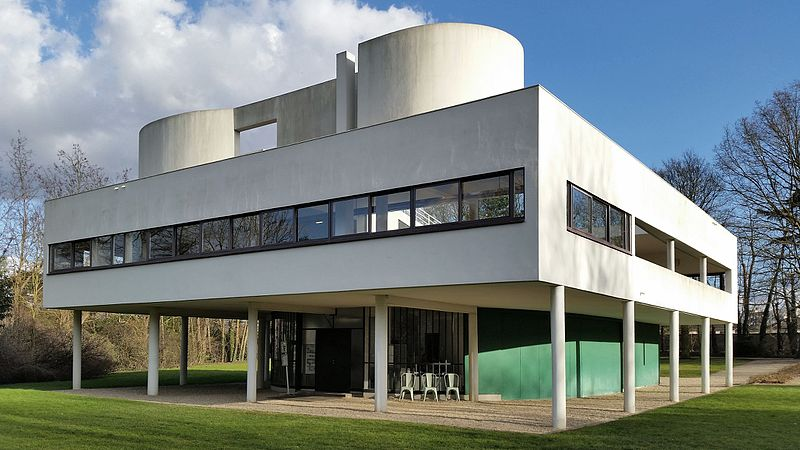
\includegraphics[height=9.85em]{chapters/fig/columns-savoye.jpg}\quad\\[1em]
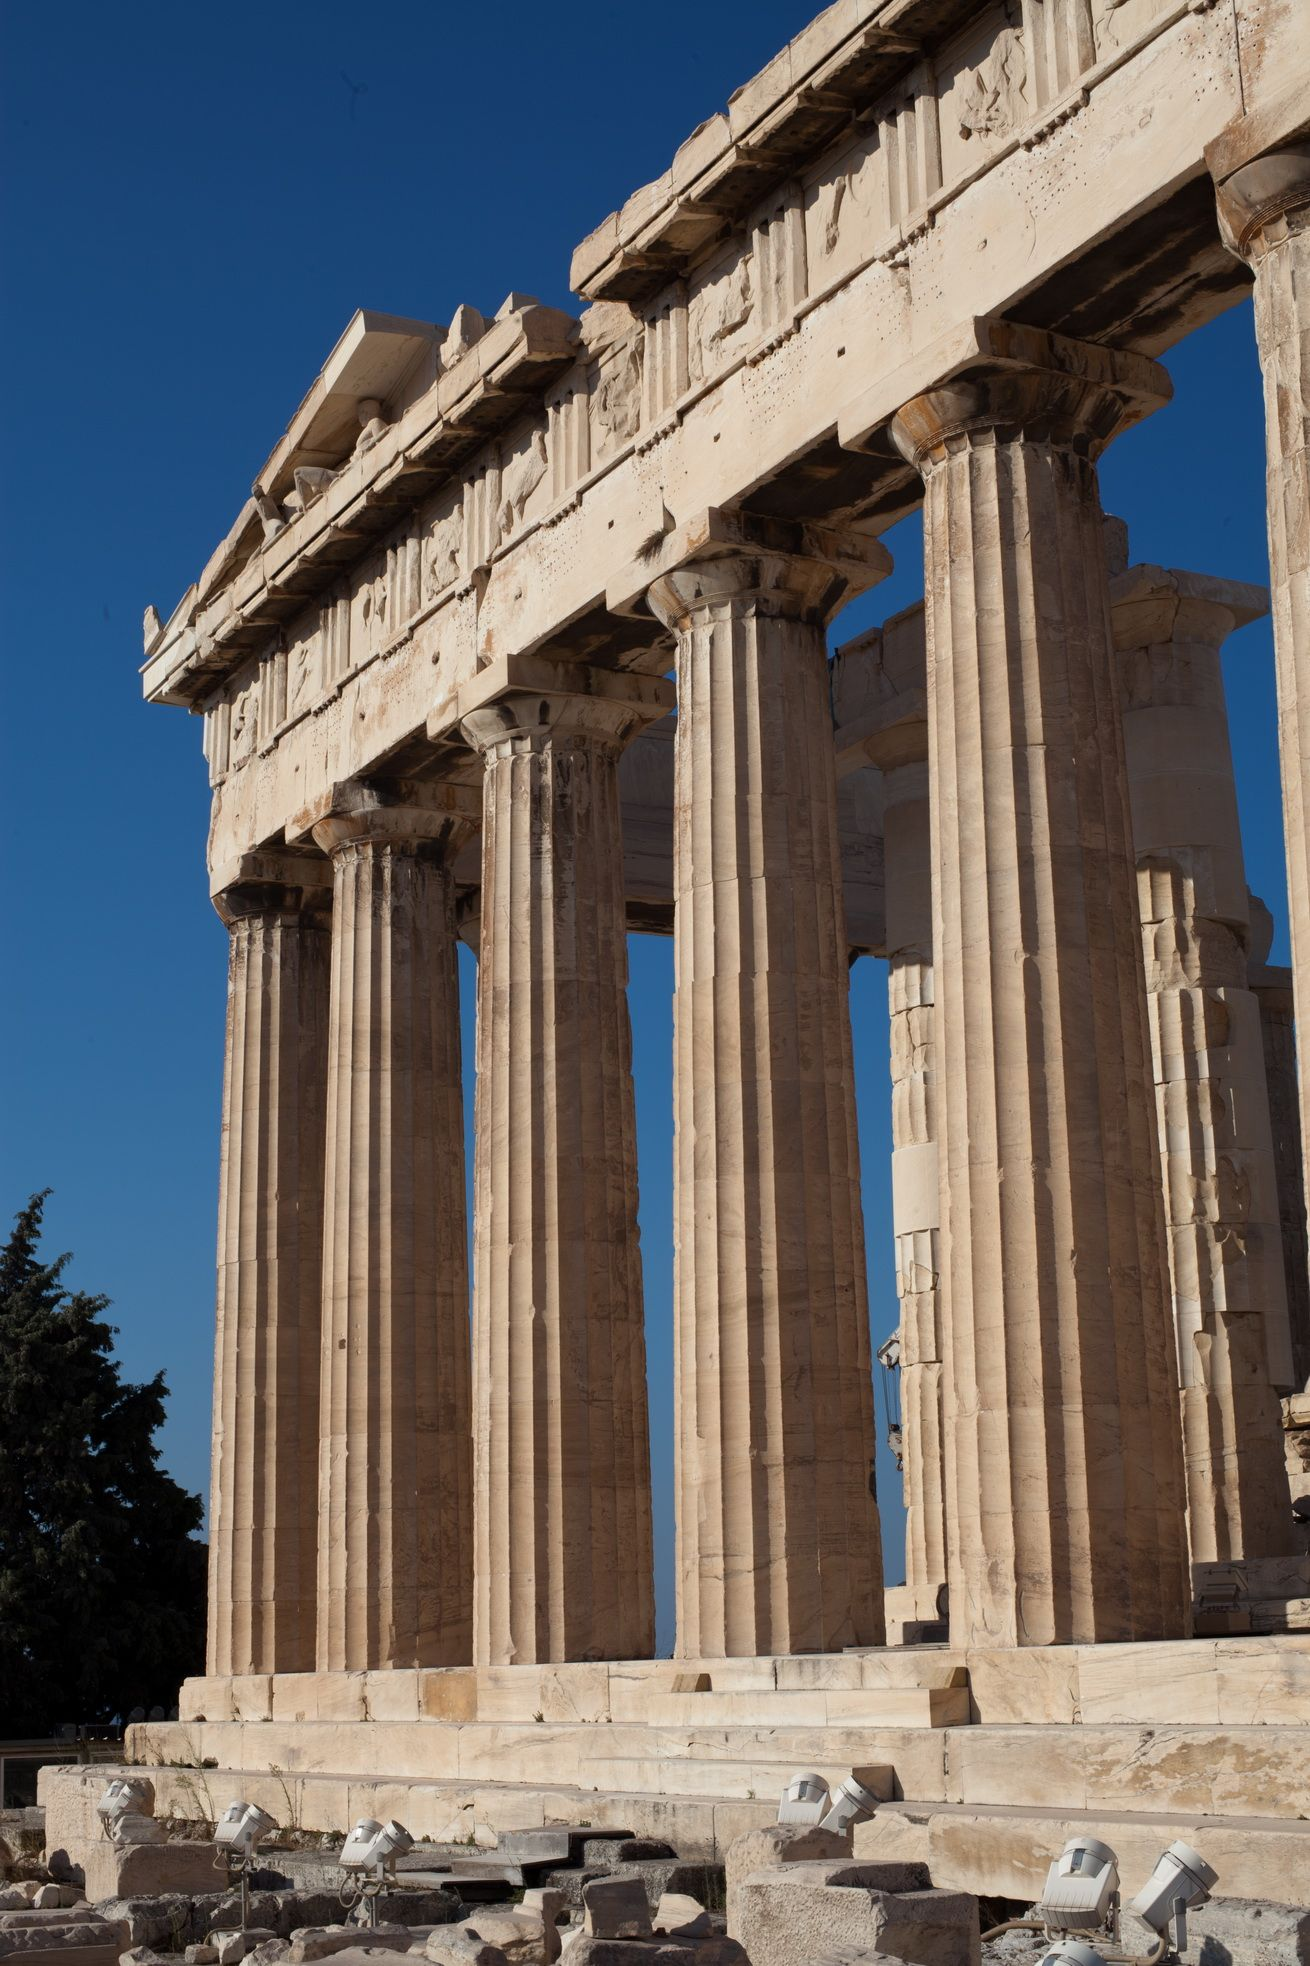
\includegraphics[height=12em]{chapters/fig/columns-greek.jpg}\quad
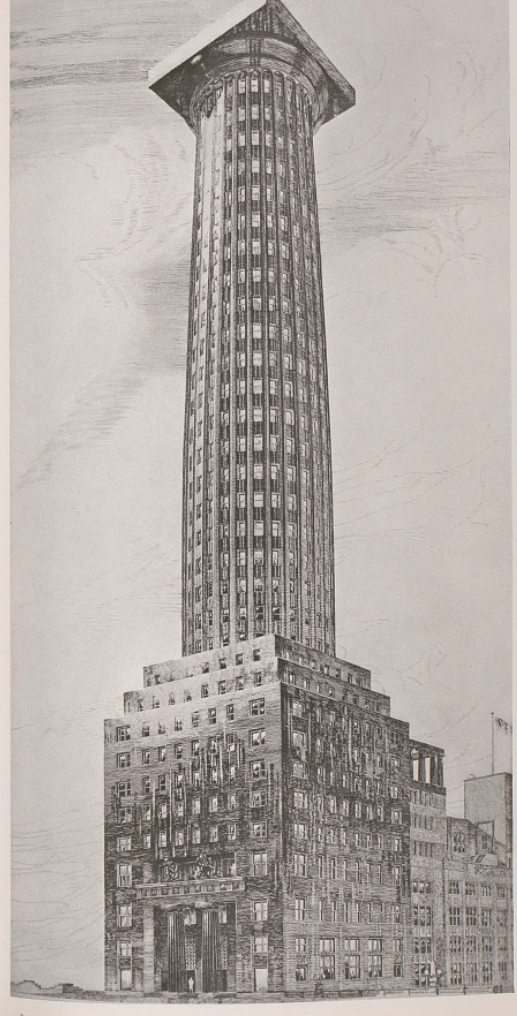
\includegraphics[height=12em]{chapters/fig/columns-loos.png}\quad
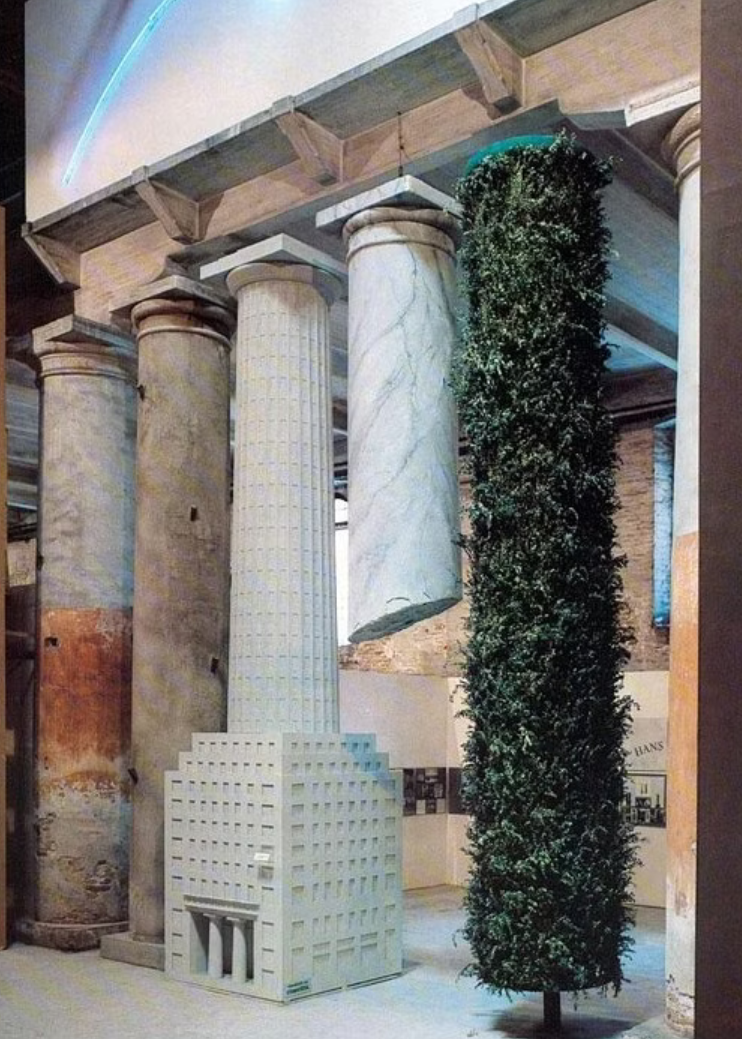
\includegraphics[height=12em]{chapters/fig/columns-venice.png}\quad
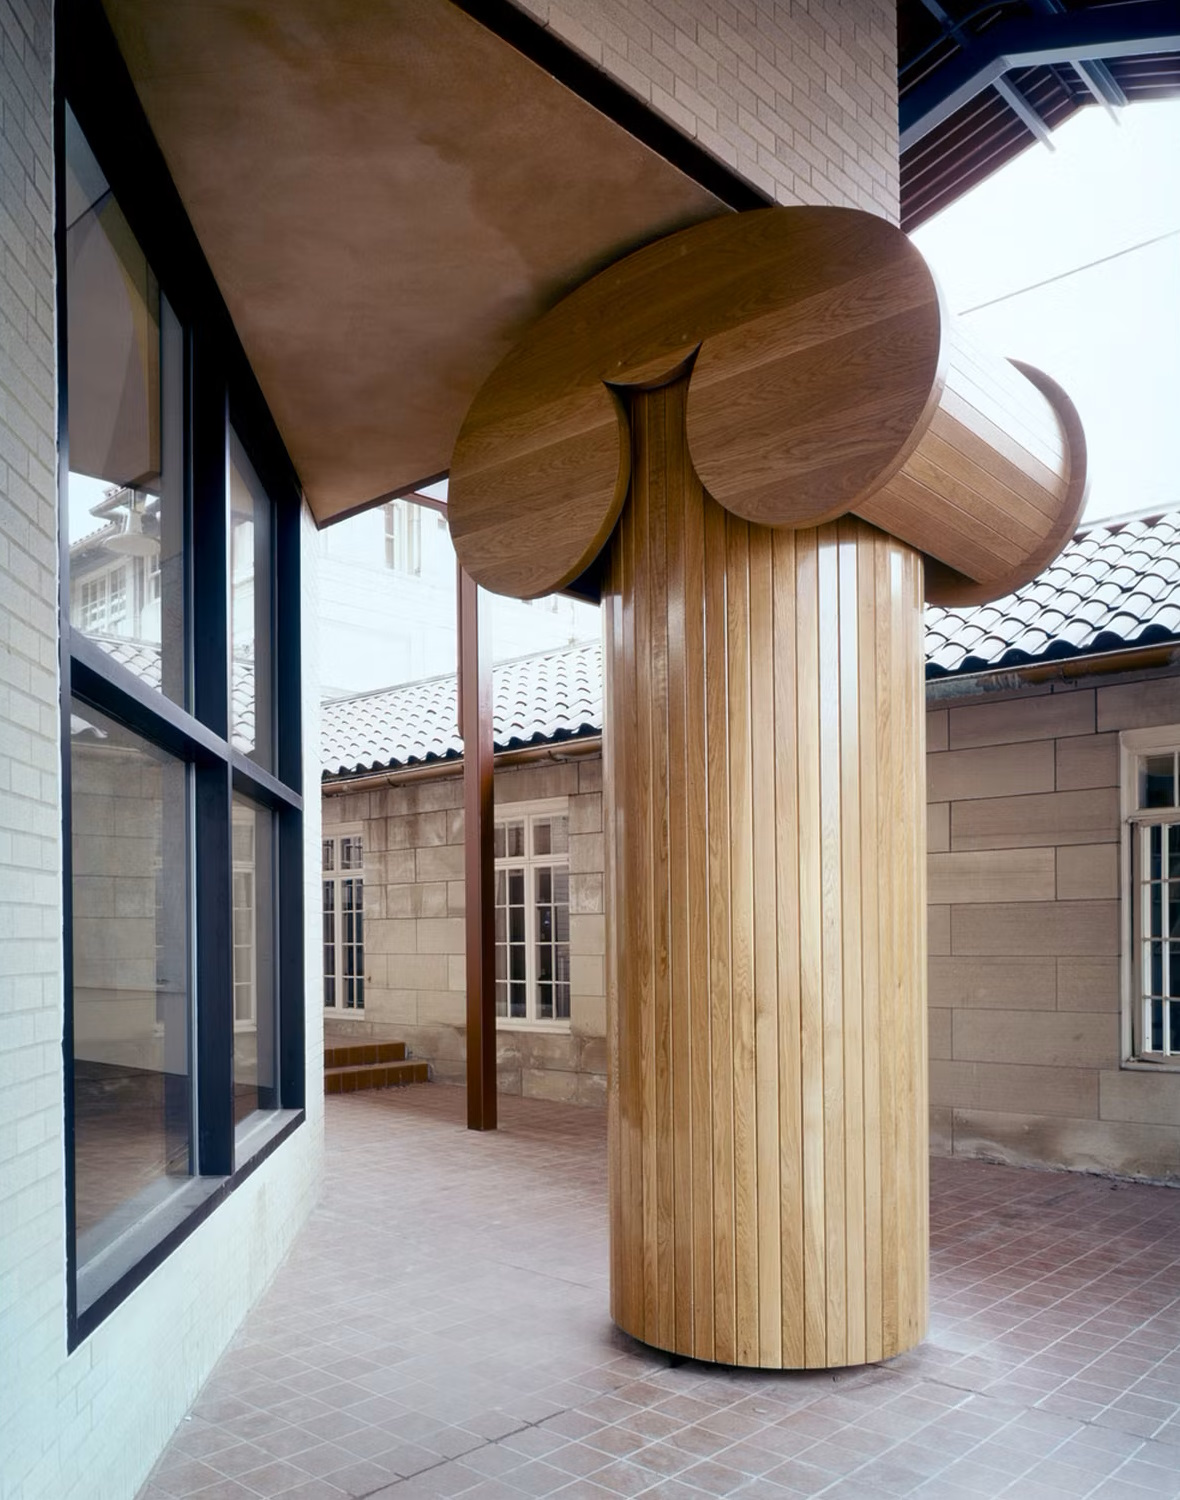
\includegraphics[height=12em]{chapters/fig/columns-venturi.jpg}
\caption{Six different uses of columns in architecture. (1) Unironical use of the column in the 1935
neoclassical building of the US National Archives, (2) Supporting pilotis in Le Corbusiers 1931
Villa Savoye, (3) The Parthenon in Athens built in the 5th century BC according to the Doric order
(4) Adolf Loos' playful reference to the Doric column in a 1922 entry for the Chicago Tribune
Tower Competition, (5) Hans Hollein's ironical Facade of Morphed Columns, at the 1980 Venice
Architecture Biennale, and (6) Robert Venturi's ``ironic'' column from the 1977 addition to the
Allen Memorial Art Museum.}
\label{fig:columns}
\end{figure}

\section{The Ironical Column}
To illustrate some of the ways through which architects use architecture to communicate, I start
with the most basic structural element of classical architecture, the column. Figure~\ref{fig:columns}
shows several uses of columns, starting from the ancient Parthenon built in Athens in 5th century
BC (bottom left) followed by four examples that include a variety of references to the classical
column.\endnote{Idea from Oppositions p377, See also Korman ``The Architecture of the Facade'' -
for more on columns}

Neoclassical architecture, which gradually grew in prominence in the late 18th century, looks
back to the Classical past. It sees it as a source of pure geometric order with ideal proportions
and symmetry. Such references to the ancients should not be unexpected. At the start of the 17th
century, Aristotle and other ancient philosophers were seen as the source of truth that was partly
lost and needs to be recovered, but that was already fully known to the ancients.\endnote{Wootton}
The scientific revolution of the 17th century gradually changed perspective on the ancients in what
was becoming experimental science, but it should not be a surpirse that architects of the 18th century
were still looking back to ancient structures that were becoming rediscovered and better understood
at the time. Neoclassical architecture remained influential after the 18th century, but its meaning
slowly shifted. It turned from an attempt to rediscover and recreate simple, purely geometrical
structures to an idealized style that emphasises tradition. The use of the style for many US federal
buildings is thus a reference to the values that the style encompasses.\endnote{Also conservative
``Executive Order on Promoting Beautiful Federal Civic Architecture'' -- Trump's administration (2020)}

The modernist Villa Savoye designed by Le Corbusier also looks back to the Classical past,
but it does so in a different way. Rather than directly copying the style and order of the
ancient Greek temples, the building is a reinterpretation of the ideas of a Greek
temple.\endnote{Unwin - Twenty-Five Buildings Every Architect Should Understand}
It reimagines the ideal structure of Greek temple based on geometric principles (using the golden
ratio), but replaces ancient Greek columns with minimalistic modernist pilotis. Following the
modernist focus on function, Le Corbusier's design uses pilotis to give prominence to the
automobile (parked on the ground floor). Although the same historical reference is present in Villa
Savoye, it is used at a more conceptual level and is not immediately apparent.

The importance of the column as an icon representing a certain style of architecture was well
understood by other modernist architects, including Adolf Loos who is best known as the author
of the modernist manifesto ``Ornament and Crime'', first presented as a lecture in 1910. In his entry
for the Chicago Tribune headquarters competition in 1922, Loos made yet another reference to the
ancient Greek temple and shaped the entire building as a giant Doric column.  Loos himself did not
view the column in his design as ornamental and instead saw it as supporting the public nature of
the building with appropriate symbolism.\endnote{Krul - Adolf Loos and the Doric Order}
The structure of the building itself here becomes the symbol in a way that is reminiscent
of later post-modernist works where construction patterns and material textures themselves become
ornament.\endnote{Jencks, p183} Despite being rooted in the modernist thinking, the Chicago Tribune
Tower project became an inspiration for later post-modern architects who make, more or less subtle,
historical references in an ironic way. They will include columns in their buildings to indicate
that they recognize being a part of architectural culture and tradition, even if they no longer
need columns as structural support mechanisms.

A good illustration of the ironic reference is the facade created by Hans Hollein for the 1980
Venice Biennale. The event took place in Corderia of the Arsenale, a large historical building
itself featuring supporting columns. The participants of the Biennale were asked to design a
facade for their exhibition that would cover (and hide) the historical structure of the Corderia.
Hollein did the exact opposite. He complemented two columns of the Corderia with a range of
ironical forms of columns. One was a bushy tree cut into the shape of a column, while another was
a scaled-down version of Loos' Chicago Tribune Tower. The entrance into the exhibition was under
a hanging fragment of a column, which clearly lost its original structural function, but gained
a different function as an exhibition entrance. Here, the ironical use of the architectural
language is direct and understandable.\endnote{Branscombe - Hans Hollein and Postmodernism}

Hollein's entry addressed the theme of the Biennale, ``The Presence of the Past'' in a way that
is funny and ironic, but sends a clear message about history and continuity of architecture. It
also illustrates the changing function of a column from supporting structure to a decoration. Moreover,
the ironical style of the presentation, shared with many other post-modern architectural works, makes
the message accessible and engaging for broader public. Hollein's facade is interesting for
yet another reason. It uses architectural language to communicate architectural ideas, but it
is neither text, nor a building. As we will see repeatedly, built structures such as stage sets
or monuments are often interesting media through which critical architectural ideas can be
expressed.

The column takes yet another form in the addition to the Allen Memorial Art Museum designed by
Robert Venturi in 1977. The extension itself is based on an idea that Venturi refers to as
the ``decorated shed''. The basic structure and spatial disposition of the building itself is
simple and serves its function which was, in part, to provide more storage space.
Any symbolic, cultural and aesthetic meaning is provided ``by modifying the basic shell by means
of design decisions of a second order.''\endnote{Oppositions, p182} One such second-order
decision is the addition of isolated iconic elements, such as the mock Ionic column that
marks the building as cultural institution. In a way, the column serves similar role as the
neoclassical architecture of the US National Archives, but is here added merely as an ironic
decoration. The association of ancient Greek columns with important public buildings remains,
but the story is told in a very different way.

% ~
%
% ~
%
% "Classicist tropes estranged from traditional use" - Aureli
%
%
% ironic historical reference - critical of neoclassicism
% change of function, repurpose
% exhibition - stage set / pavilons, allows for communication
% reveal inherent conflicts
% ironically distort regularity - point out things
% change of function - non-structural (decorated shed)
% irony valued for superior depth, allows showing multiple contradictory views (Jencks, 79)
% intellectual reference to other works vs. funny reference for broader public - to engage with wider audience!

\section{Towards Critical Software}

In my attempt to translate the critical langauge of architecture into the world of software,
I will alternate between two modes of working. First, I will reinterpret existing practices
in software development and computer science in light of the architectural theory. Second,
I will suggest how we could more deliberately follow in the footsteps of architects and
create new software artifacts that express critical points about software.

In other words, can we follow post-modern architects and embed criticism as a first-class
element in software practice, rather than leaving it to a second-class (and largely optional)
critical writing?\endnote{Oppositions 377, also Venturi introduction} We can also look to
post-modern architects for initial ideas of what such critical software can say. The
architectural style known as eclecticism makes funny references such as Hans Hollein who
decorated his Austrian Travel Agency office with metalic palm trees and broken Greek
column.\endnote{Jencks, p56} The appeal of the style is not just its straightforward humour,
but the fact that it is understandable and can communicate with wider audience. Similarly,
post-modern architects have used contextualism to highlight important characteristics of the
environment they work in or use references to suggest alternative social organization.

Looking at existing software practices, we can imagine how the above arhictectural ideas
can apply to basic structural elements from which software is built. One such element may
be the data structures around which software is structured.\endnote{ref Abstracting craft p96;
ref Joel - the other part of the basic structure is how change is described} Data structures
in software are arguably even more fundamental than columns in architecture, because any
software that works with data needs to store the data in some way. The limitation of this
metaphor is that, unlike columns which are typically visible, data structures are typically
hidden from the end-user. There also is no singular classical model of data structures,
although a number of models fit a similar role. These include the relational model of databases,
flat memory model of low-level programming languages and data types that model data as collections
of nested records.\endnote{Memory models blog}

We can use the architectural metaphor to talk about the differnt kinds of classical models
of data structures. Whereas the relatively expressive language of the relational model or
the nested records model could be linked to different kinds of classical columns, the minimalistic
models of flat memory or nested lists of the Lisp programming language are more akin to
modernists undecorated and purely functional pilotis.

When the data structures are used to store data, they serve the original intended purpose,
just like columns functioning as supporting structure. But equally, there are software systems
where data structures are used more as rhetorical elements, intended not for the computer
execution of the software, but for the end-user or programmer. One example would be types
in the TypeScript programming language. Here, the actual representation of data can be anything
permitted by the underlying JavaScript runtime. TypeScript type declarations are mere labels,
intended for the human and for the static TypeScript type checker, but they are not enforced or
used for checking at runtime. The type declarations still look like a definition of the shape
of a data structure (a column), but they no longer play the basic structural function. They are
used for paratial checking (a scaffolding around a column?) and as information for the
programmer (a purely rhetorical column). A similar case would be the use of data structures
in non-relational databases such as key-value stores or document databases. The data stored
in such systems in practice has some implicit structure.  However, any explicit description
of the structure is merely literal. The description may use the language of standard data
structures (collections, records, primitive types), but this is not used for representation.

Do certain data structures also have particular symbolic associations, in a manner similar
to how the Classical column stands for traditional values, often associated with US federal
buildings? I believe this is the case. For instance, the class-based object-oriented
programming paradigm is often associated with maintainability. Languages that adopt
class-based object-oriented abstractions as their basic data structure do not do so
just for practical, but also for symbolical reasons. TypeScript serves to illustrate this
again. One of the first books on the language claims that ``TypeScript [brings] a level of
maintainable structure to JavaScript development through its class and module
features.''\endnote{Dan Maharry, TypeScript Revealed, 2013} Written in the same year when
the language was released, the claim could not rely on empirical experience with the language,
but mainly on the symbolic associations of the data structure.

\begin{figure}
\begin{lstlisting}[language=csxml]
<CsamlFile xmlns="http://schemas.microsoft.com/winfx/2006/xaml/csaml"
      xmlns:x="http://schemas.microsoft.com/winfx/2006/xaml">
  <NamespaceDeclaration Identifier="MyNamespace">
    <ClassDeclaration Identifier="MyClass" Access="Public">
      <MethodDeclaration Identifier="Main" Access="Public"
            Modifier="Static" ReturnType="{x:Type void}">
        <InvocationExpression MemberAccess="System.Console.WriteLine">
          <InvocationExpression.ArgumentList>
            <Literal Type="{x:Type string}" Value="Hello, CSAML!">
          </InvocationExpression.ArgumentList>
        </InvocationExpression>
      </MethodDeclaration>
    </ClassDeclaration>
  </NamespaceDeclaration>
</CsamlFile>
\end{lstlisting}
\caption{The ``Hello world'' program written using the C\# Application Markup Language (CSAML),
conceived by Charles Petzold in an April Fool's post on 1 April 2006.\endnote{\url{http://www.charlespetzold.com/etc/CSAML.html}}}
\label{fig:csaml}
\end{figure}

For my last example based on a reference to an existing artefact, I want to show that
data structures have already been used to make critical ironical statements. The April Fool's
post written by Charles Petzold in 2006 introducing the ``C\# Application Markup Language''
is a illustration.\endnote{\url{http://www.charlespetzold.com/etc/CSAML.html}}
The post introduces a new notation that encodes programs written in the C\# language
using XML (Figure~\ref{fig:csaml}). The post can be seen as an ironical work of contextualism.
The post was published in the heyday of the XML format when Microsoft released multiple
development frameworks built around XML. As a well-written April Fool's joke, the post
made readers think. The post praises the semantic clarity of the XML format and gives
various examples that are extremely lengthy and tedious. After a brief puzzlement, most readers
realise the joke. But the post makes them wonder about the verbosity and unnecessary
overuse of the format at the time.

~

funny, architectural plans, esolangs

FUTURE
point out what we are doing without thinking - information hiding - expose data structures!

~

~

~

Oppositions p376

"criticism embedded in practice" (Venturi) - not just code, but also docs
Eclecticism - be funny (Jencsk) - engage with audience in a fun way?
Morality / social relevance (Jencks) - c.f. thimbl

self-referential sign
-> thing ported from (native) environment to expensiove recreation in another? (to keep UX or something?)

serious artists engage with history, choosing what to keep and what to drop (The Hub)
rebuilding old things anew?
-> reconstructions

Class as a column?
basic structure, associated with maintainability...
(evolved from closures and back)

god object / class? - chicago tribune

types and data structures - in cases where they are not enforced (nosql) - mere nice annotations
- data structure characerizes software - Craft, p96
=> vocabulary for what you can do - disrupt? nosql databases (allow anything) -
c.f. craft p98 (disrupt the gap in definining vs. understanding SW structures?)

point out things that we're doing without thinking (information hiding)
-> expose structure

Rhetorical element? (Venturi)

highlight contradictions - plenty in software
hard to read architecture is valid if it reflects contradictions (Venturi)

exhibitions / stage sets
-> format for communication
-> heterotopias (Jencks)


Deconstruction
- use some methodological way rigorously to show where it leads

\section{Eisenmann}

some theoretical analysis

\section{PL world}
https://parametric-architecture.com/deconstructing-deconstruction-the-architectural-philosophy-of-peter-eisenman/

https://arahovsepyan.com/eisenmanalexander

abstract entity to support any kind of activity (Aureli)

\section{Achieving fit?}

Modernism, Vegas, Alexander


\newpage

HOW CAN IT BE DONE

manipulate language / formal codes - oppositions p376

self-referentiality to build more meaning
  (risks danger of intellectualism)

contrast double coding - one meaning for the building, one for the viewer
(one for computer, one for the human)

metaphorical operation (grid c.f. abstraction!
  relate grid in city with grid in floorplan cf oppositions)

operate on codes (Oppositions 377, c.f. chicago column)

use pavilons/stage sets to show what capitalism has
taken away from us on a small scale
c.f. heterotopias (Jencks)

performative science fiction

what can house/software express besides its function?

see Oppositions 376

more methodological freedom!
(build silly things; needed for deconstruction etc.)

eclecticism? pop? learning from las vegas?

PM liberated communicative potential - dtto! (Jencks)

! need to see inside things, which is why programming systems perspective matters
(in a house, you can talk through the internal structure, as long as it functions)

but SW is more than code - also docs etc. - take broader perspective!
(community etc.)

monuments / demoscene / esolangs / talks / hackathons
(building as ritualistic activity to encourage social bonds - Aureli)

\section{Leftovers}

POP/LAS VEGAS
Sources for new socially relevant language (Oppositions 329)
(Oppositions, 656,  667)
discussion - learning from las vegas
vs. should speculate what society should be


THREE EXAMPLES FOR INTRO
* something formal geometrical (abstract)
  - abstraction
  - more followers of modernism
  - memorial
  - pinwheel bauhaus building - formal mirrors school strcutrue (Eisenmann thesis last chapter)
  - plazas become ice skating rinks (no need for functional motivation, Oppositions 67)
* something post-modern - saying things with architecture
* chiat
* deconstruction?
*


maybe one monument?

INTRODUCTION
* Alexander's hired guns
* limited options of architect (Jencks?)
* we lack the language for answering alexander's question
* New glass architecture must wrench the European out of his coziness (Oppositions, 55)
* c.f. architecture as bloodless pseudo-science (Oppositions, xii)
  totaliarization of technique (Frampton) - how to escape?
* irony (operate in a system to which one is critical)
* structure that enables things (Venturi, 13; Tufekci)
* social visions - but how to phrase? plans, monuments
* learning from - las vegas (or opposing it; Oppositions 656); manhattan
* \#1 - eisenman (deconstruction)
* \#2 - postmodern (speaking)
* \#3 - venturi - what is vs. what should be


% ==================================================================================================
% CHAPTERS
% ==================================================================================================

SPACE/NAVIGATING
* inhabiting, terrain vague, navigating in systems

MATERIALITY
* looks bad before goes bad
* materials - become ornament (Jencks, 183)
* material honesty (Depaz)

ACHIEVING FIT
*

ORNAMENT
* decorated shed - typescript, structure becomes ornament - APL

ABSTRACTION
* as arising from human world?
* we deny that abstraction is a reflection of larger historical and cultural forces (Aureli, vii)
* abstractions are concrete, emerge from tangle of human actions (Aureli, ix)
* not due to strucutre, but due to the way it is produced (division of labor, etc.) (Aureli, x)

COMPLEXITY
* Jacobs, Venturi (Jencks, 116)

SELF-REFERENTIALITY
* "shapes that do not refer to something else (just other shapes)" (Oppositions, 205)
* return to language (Oppositions, 373); layers of signification
* LANGUAGE, GRAMMAR

POST-MODERNISM
* complexity, plurality of meaning (Venturi) - as reaction to modernism (Oppositions, 202)
* a mechanism for critically reflecting on history
  (c.f. column with gap as decoration; reverse meaning)

DECONSTRUCTION
* deconstruct all methodologies without replacing them with a new one
  (but Derrida's criticism of Eisenmann in Chora L Works)

GRAMMAR
* Bruneleschi - origins (Aureli) - enables "building out of time"
* c.f. Eisenmann

SELF-REFERENTIALITY / LANGUAGE / DECONSTRUCTION II
* fully abstract - how buildings enclose space (Aurelli)
* fully abstract in that it forces no specific use (Co-op interior)
-> how much structure SW forces on us?

PLANS / MONUMENTS
* cf. Aureli


SLOW SOFTWARE

Cartesian grid as first class - reveal technique
-> political significance of the grid (Aureli); challenge reading grid as rational system
mis-leading axonometric drawings (Eisenmann)
-> plans as the device (does not have to be built)
basic L shape as critique of modernist simple building blocks
-> DECONSTRUCTION

\theendnotes
